\chapter{Testy}
\label{cha:testy}

Dla potrzeb symulacji zostały stworzone trzy mapy przedstawione w~poniższej tabeli (Tabela \ref{tab:mapy}). Pozycje pieszych były odświeżane w interwale $100 ms$ co pozwoliło na realistyczne odzwierciedlenie ruchu. \\

\section{Wyniki}
\label{sec:wyniki}

Wszystkie rysunki oraz wykresy zostały przedstawione poniżej oraz w dodatku A dla przejrzystości.\\

\begin{tabular}{c||c|c|c|c}
\label{tab:mapy}
\caption{Porównanie parametrów symulacji}
/ & Mapa & Ilość pieszych & ilość wystąpień czekania & czas symulacji \\ 
\hline 
1 & Wąskie gardło 1 & $20$ & $186$ & $61,982 s$ \\ 
2 & Wąskie gardło 2 & $50$ & $235$ & $68,961 s$ \\ 
3 & Wąskie gardło 3 & $70$ & $1681$ & $73,473 s$ \\ 
5 & Lejek 1 & 20 & $170$ & $65,372s$ \\
6 & Lejek 2 & 50 & $826$ & $67,133s$ \\
7 & Lejek 3 & 70 & $1384$ & $69,729s$ \\
8 & Labirynt 1 & 20 & 254 & $76,030s$ \\
9 & Labirynt 2 & 70 & 345 & $82,034s$ \\
\end{tabular} 

Nawiązując do tabeli \ref{cha:testy} porównane zostało dziewięć map różniących się ułożeniem przeszkód oraz ilością pieszych. 

Podsumowując wszystkie wykonane testy można zauważyć sporą ilość wystąpień czekania. Jest to liczba mówiąca o~ogólnej ilości wystąpień zjawiska czekania na całej mapie podczas całego czasu działania aplikacji. Liczby są dość spore głównie za sprawą sposobu implementacji symulacji. Zaproponowany w pracy sposób nie zakłada obliczania nowych ścieżek dla pieszych, którzy zmienili swoją bazową pozycję za sprawą działających nań siły. Zostały podjęte takie próby, jednakże za sprawą niskiej wydajności takiej symulacji autor zdecydował się na zaniechanie prac w tym kierunku. Pieszy po zmianie swojej pozycji względem ścieżki bazowej próbuje do niej powrócić. Po wystąpieniu kolizji w~pierwszej kolejności podjęta zostaje próba zmiany prędkości lub jej kierunku, jeśli działanie to nie zakończy się sukcesem pieszy musi się zatrzymać, aby nadal podążać swoją ścieżką.

Długość czasu symulacji informuje nas o całkowitym czasie potrzebnym do opuszczenia mapy przez wszystkich pieszych. Ma to szczególne znaczenie w przypadku kiedy rozpatrujemy przypadek ewakuacji, możemy w~łatwy sposób dowiedzieć się ile będzie ona trwać. \\

- \textit{wąskie gardło 1, 2, 3} - Można dostrzec duże różnice pomiędzy $20$ agentami oraz ich większą ilością. W~pierwszym przypadku nie obserwujemy dużego zagęszczenia tłumu przy wejściu do przewężenia. Oczywiście w~środku oraz w okolicach wyjść gęstość znacząco wzrasta co jest zgodne z oczekiwaniami. W~przypadkach dla $50$ oraz $70$ pieszych dostrzec można dużo większą gęstość przy wejściu do przewężenia oraz znaczące zawirowania w ruchu pieszych co jest naturalne ze względu na występowanie większej ilości sił pomiędzy nimi. W~przypadku~2 oraz~3 gęstość jest niższa w~okolicach wyjść co koreluje z mniejszą ilością pieszych przedostających się jednocześnie przez przewężenie.

Wartym zwrócenia uwagi jest fakt czasu przejścia pieszych przez mapy.~W przypadku $20$ pieszych czas jest trochę krótszy~w porównaniu do reszty map, natomiast uwagę zwraca także kształt wykresu. Do przejścia połowy pieszych przez mapę potrzeba krótszego, ale podobnego czasu jak~w innych przypadkach, ale czas opuszczenia mapy przez innych pieszych po opuszczeniu połowy~z nich jest również krótszy. Wykres jest bardziej ścięty niż~w reszcie przypadków.

- \textit{lejek 1, 2, 3} - w~pierwszym przypadku gęstość pieszych rozkłada się dość równomiernie. Dopiero w miejscach wyjść dostrzec można znaczący wzrost gęstości. Jest to spowodowane sporą ilością pieszych dążących do tego samego miejsca, który nie są po drodze znacząco zatrzymywani. Ścieżki ruchu są dość jednolite. Dla przypadku $50$ pieszych można zauważyć wzrost gęstości przy wejściu do zwężenia oraz przez jego długość. Znaczący wzrost może zostać zanotowany w~miejscu zakończenia zwężania - wówczas każdy z~pieszych musi wybrać jeden z kierunków podążania do wyjścia pierwszego lub drugiego co powoduje spore zawirowania. Po wyjściu ze zwężenia gęstość pozostaje na podobnym poziomie i ponownie wzrasta w miejscu wyjść. Dla ostatniego przypadku z największa gęstość przypada w miejsce wejścia do przewężenia, podobnie jak w~przypadku dla wąskiego gardła. Tutaj ponownie jest to spowodowane z dużą ilością pieszych chcących dostać się do środka. 
Ilość pieszych w czasie dla każdego z przypadków układa podobnie jak w przypadku mapy w formie wąskiego gardła.

- \textit{labirynt 1, 2} - W~obu przypadkach zanotowań można wzrost gęstości w~miejscach przejścia przez "korytarze", czyli dróg jakie musi obrać wiele pieszych w celu dojścia do wyjścia. W~przeciwieństwie do poprzednich przypadków nie notuje się znaczącego wzrostu gęstości w~miejscach wyjść. Jest to spowodowane z równomierniejszym przemieszczeniem się pieszych, a co za tym idzie mniejszą ilością osób w~wyjściach jednocześnie. Ścieżki przejść są również mniej zawirowane z powodu większej możliwości obrania dróg. Warto zauważyć, że wykres ilości pieszych w~czasie układa się inaczej niż w poprzednich przypadkach. W~szczególności dla przypadku 7 dostrzec można, że pieszy agent dużo szybciej opuszcza mapę, a~sam wykres jest mniej stromy. Jest to spowodowane większą swobodą wyboru ścieżek oraz samego ruchu pieszych.


\begin{figure}
\label{figure:siatka}
\centering
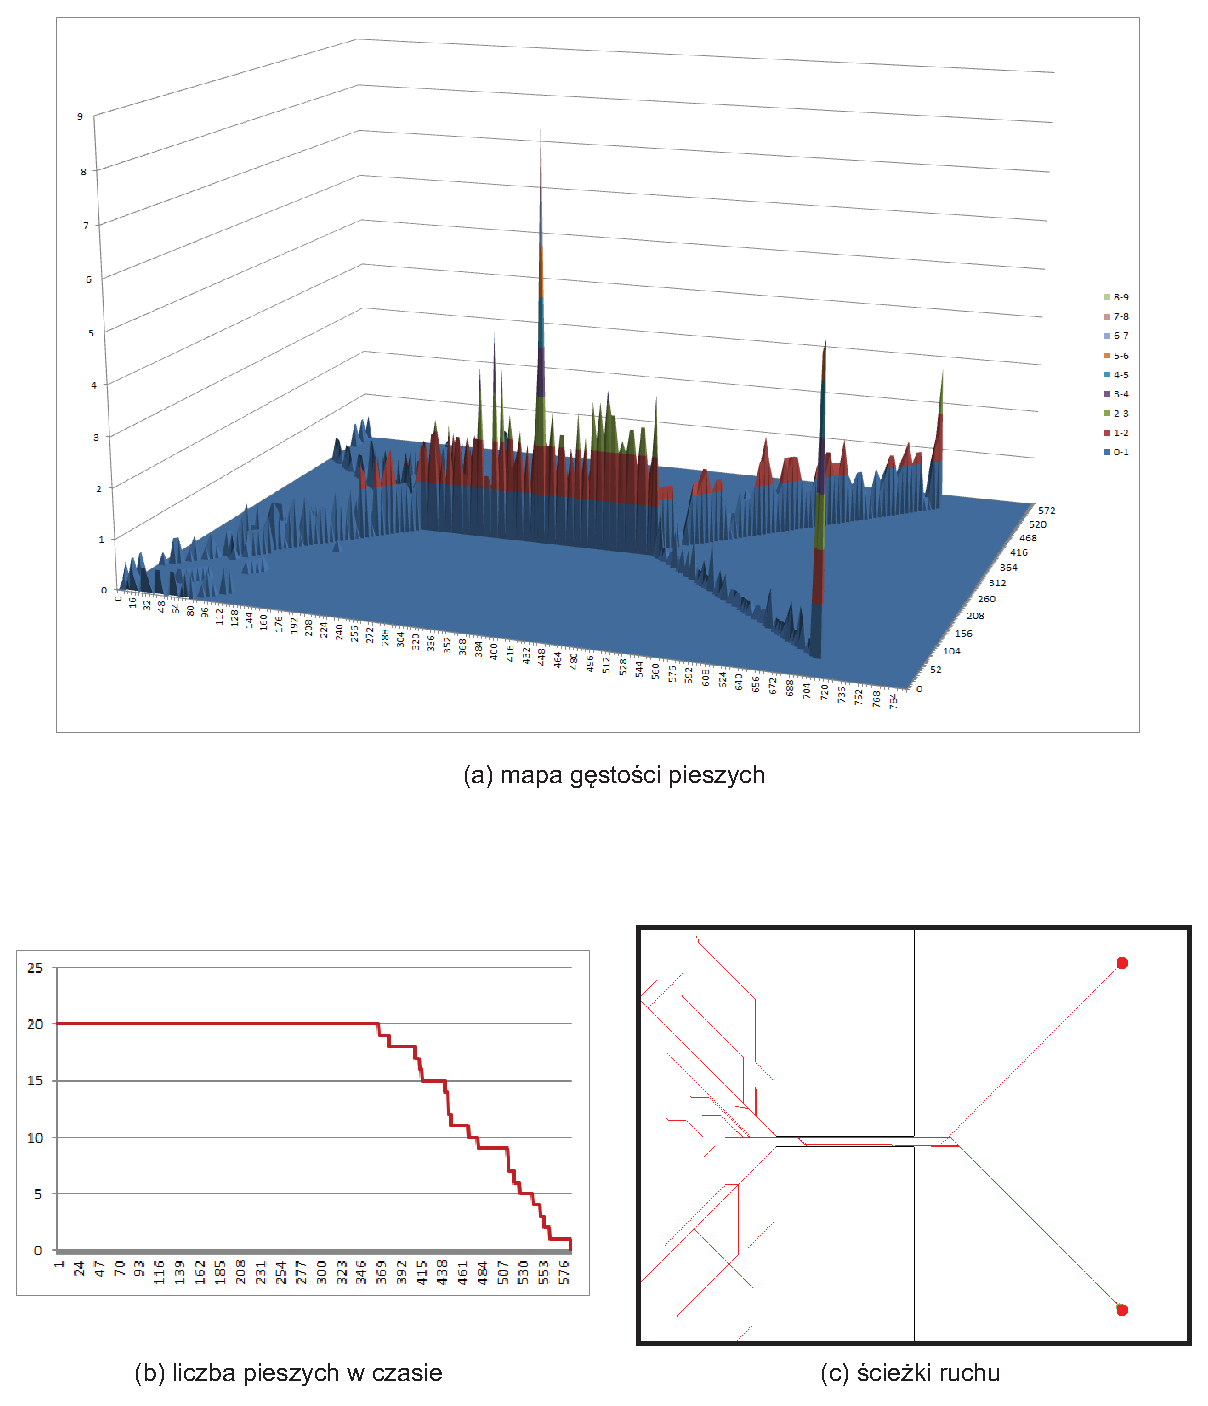
\includegraphics[width=1\textwidth]{waskiegardlo20.eps}
\caption{Ruchu pieszych podczas przejścia przez wąskie gardło dla 20 agentów, przypadek 1 (opracowanie własne)}
\end{figure}

\begin{figure}
\label{figure:siatka}
\centering
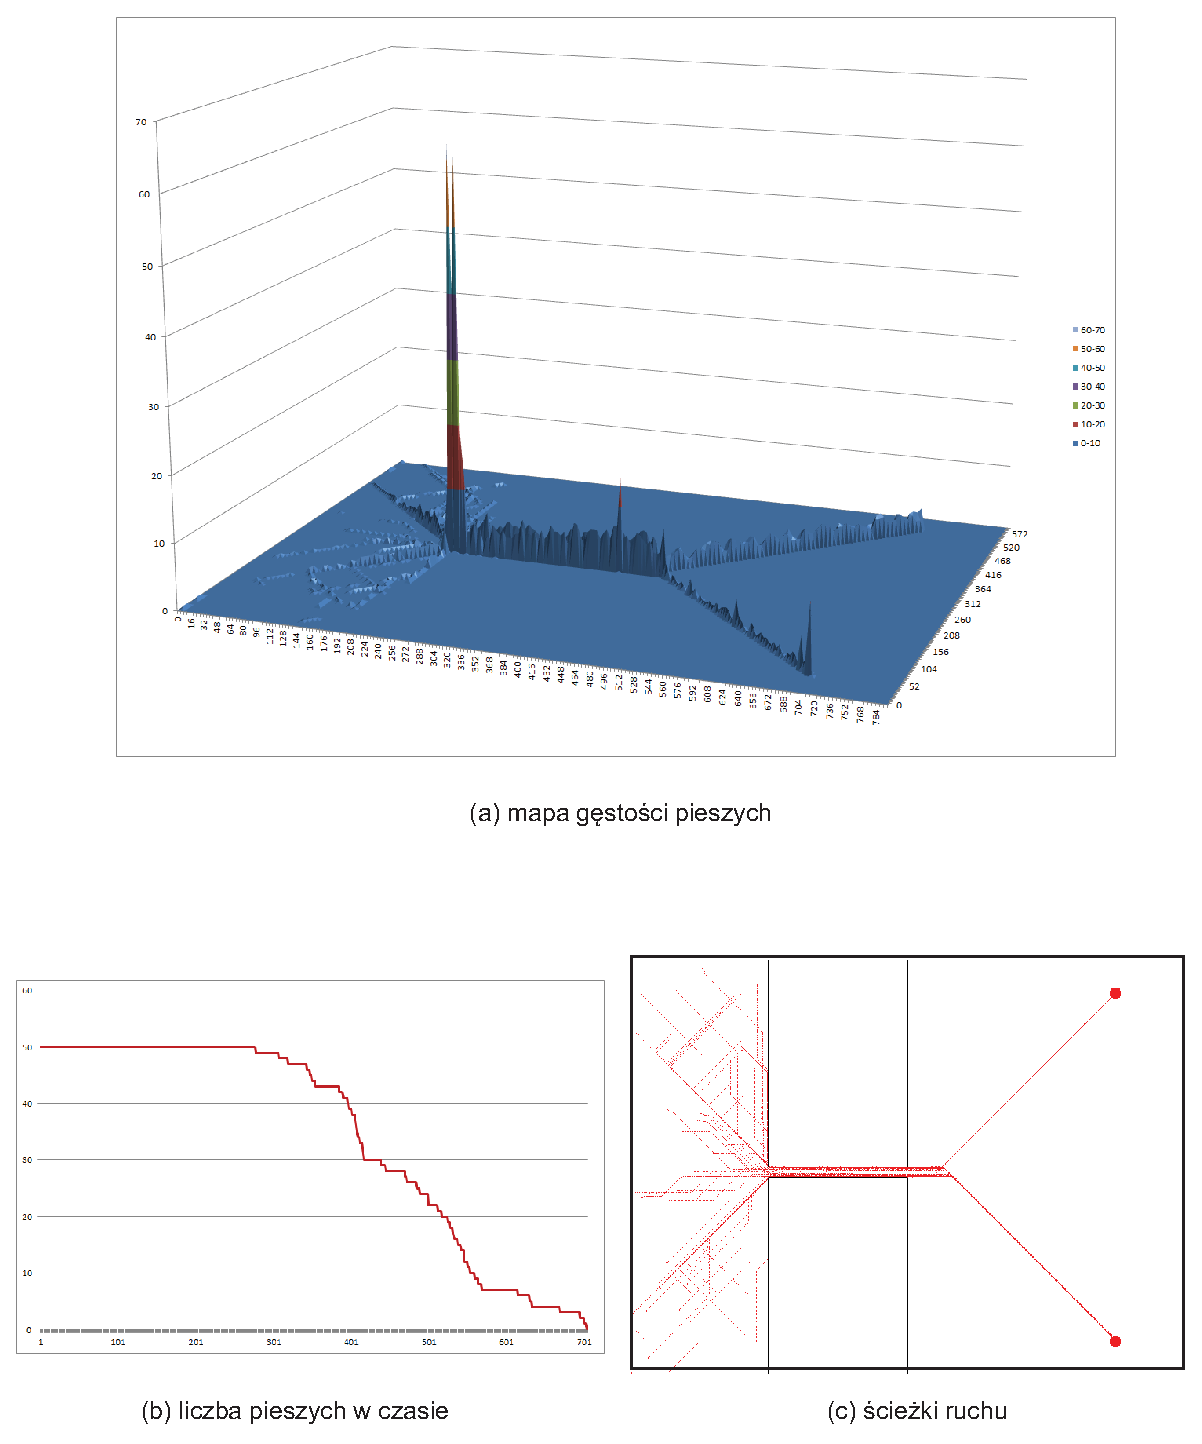
\includegraphics[width=1\textwidth]{waskiegardlo50.eps}
\caption{Ruchu pieszych podczas przejścia przez wąskie gardło dla 50 agentów, przypadek 2 (opracowanie własne)}
\end{figure}

\begin{figure}
\label{figure:siatka}
\centering
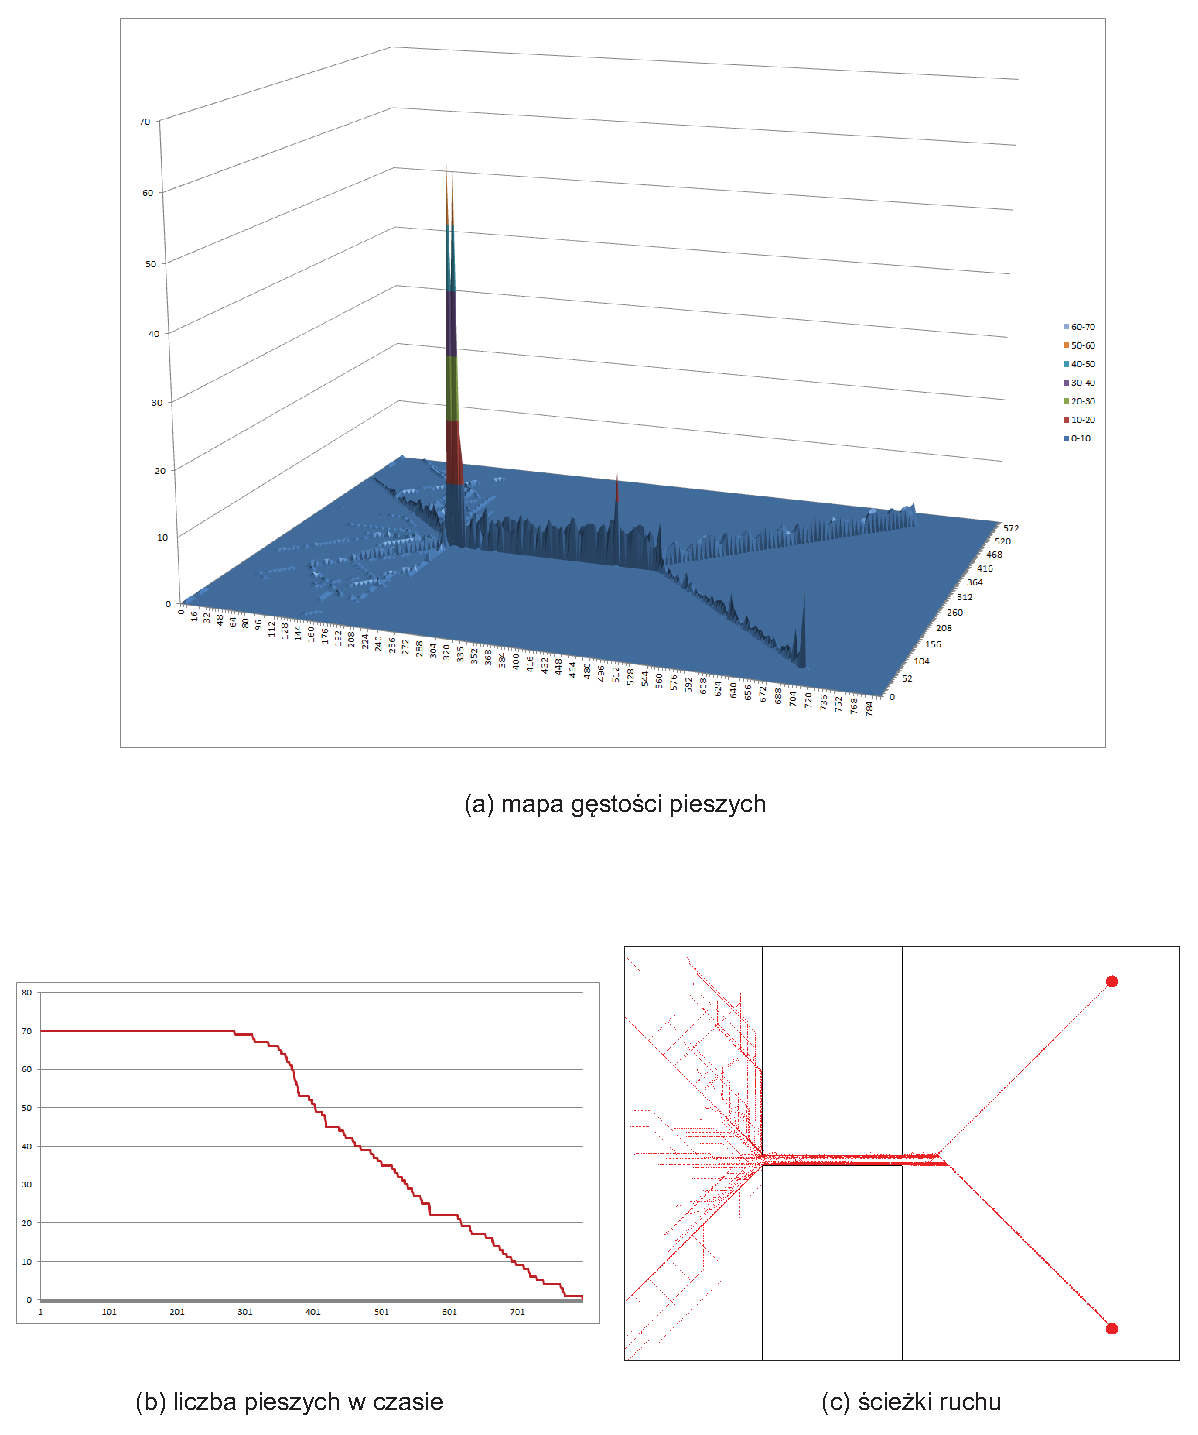
\includegraphics[width=1\textwidth]{waskiegardlo70.eps}
\caption{Ruchu pieszych podczas przejścia przez wąskie gardło dla 70 agentów, przypadek 3 (opracowanie własne)}
\end{figure}

\begin{figure}
\label{figure:siatka}
\centering
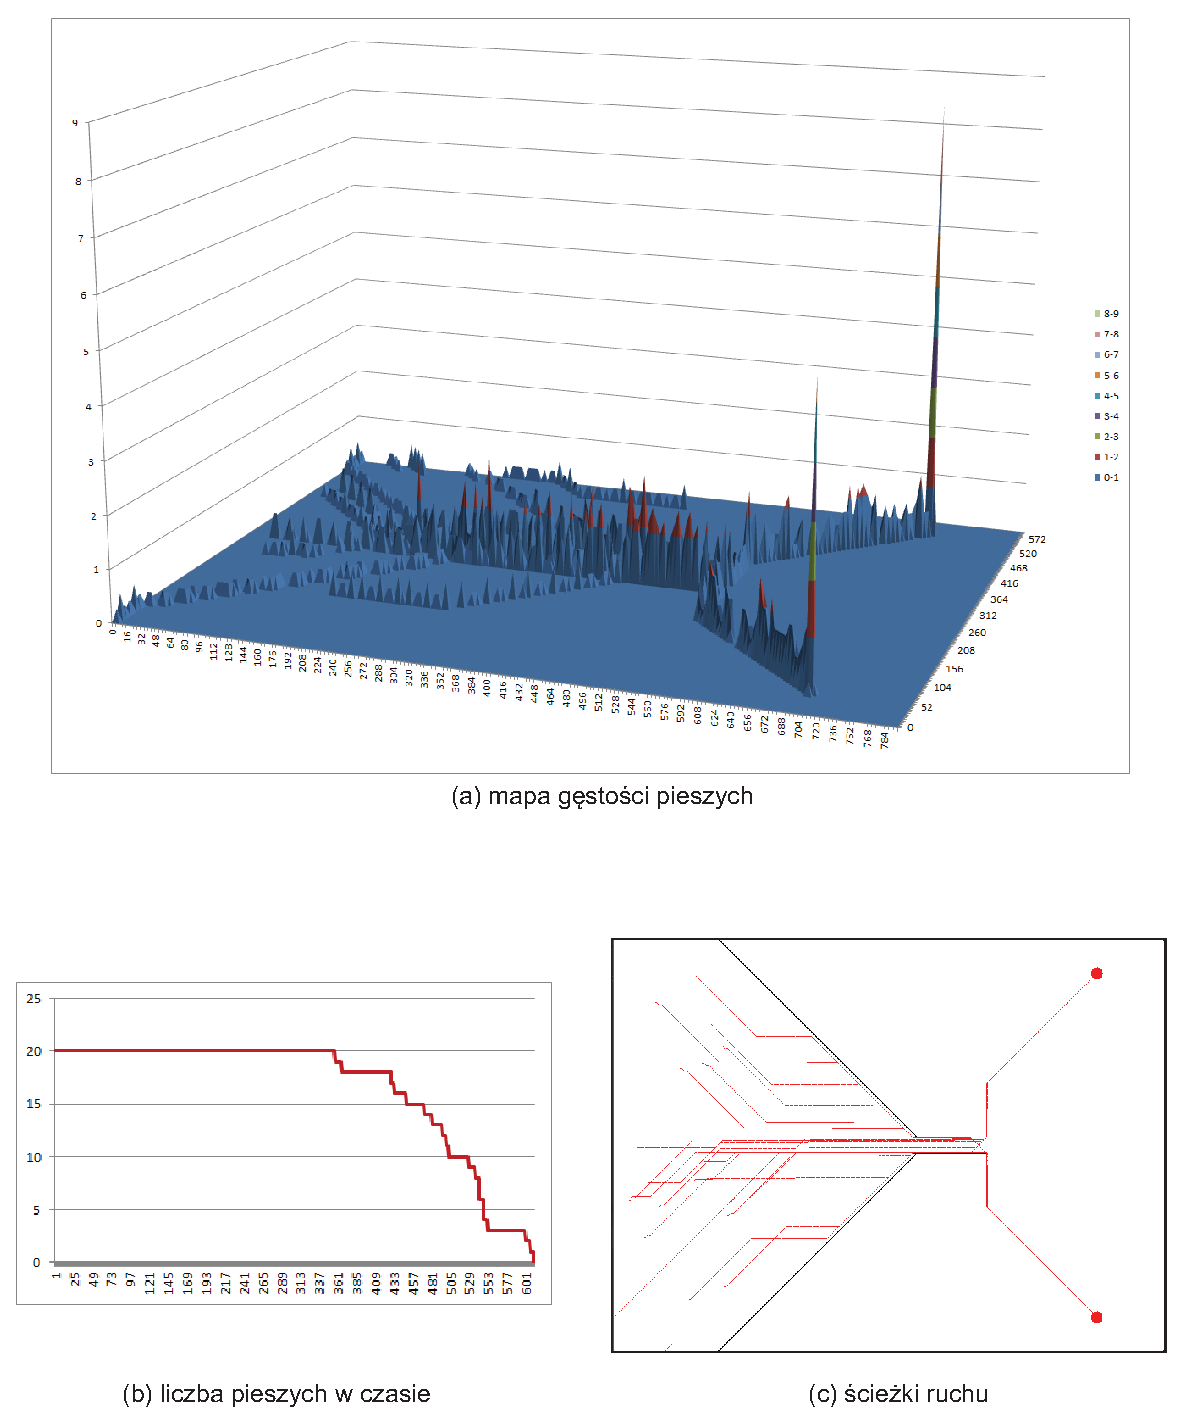
\includegraphics[width=1\textwidth]{lejek20.eps}
\caption{Ruchu pieszych podczas przejścia przez lejek dla 20 agentów, przypadek 4 (opracowanie własne)}
\end{figure}

\begin{figure}
\label{figure:siatka}
\centering
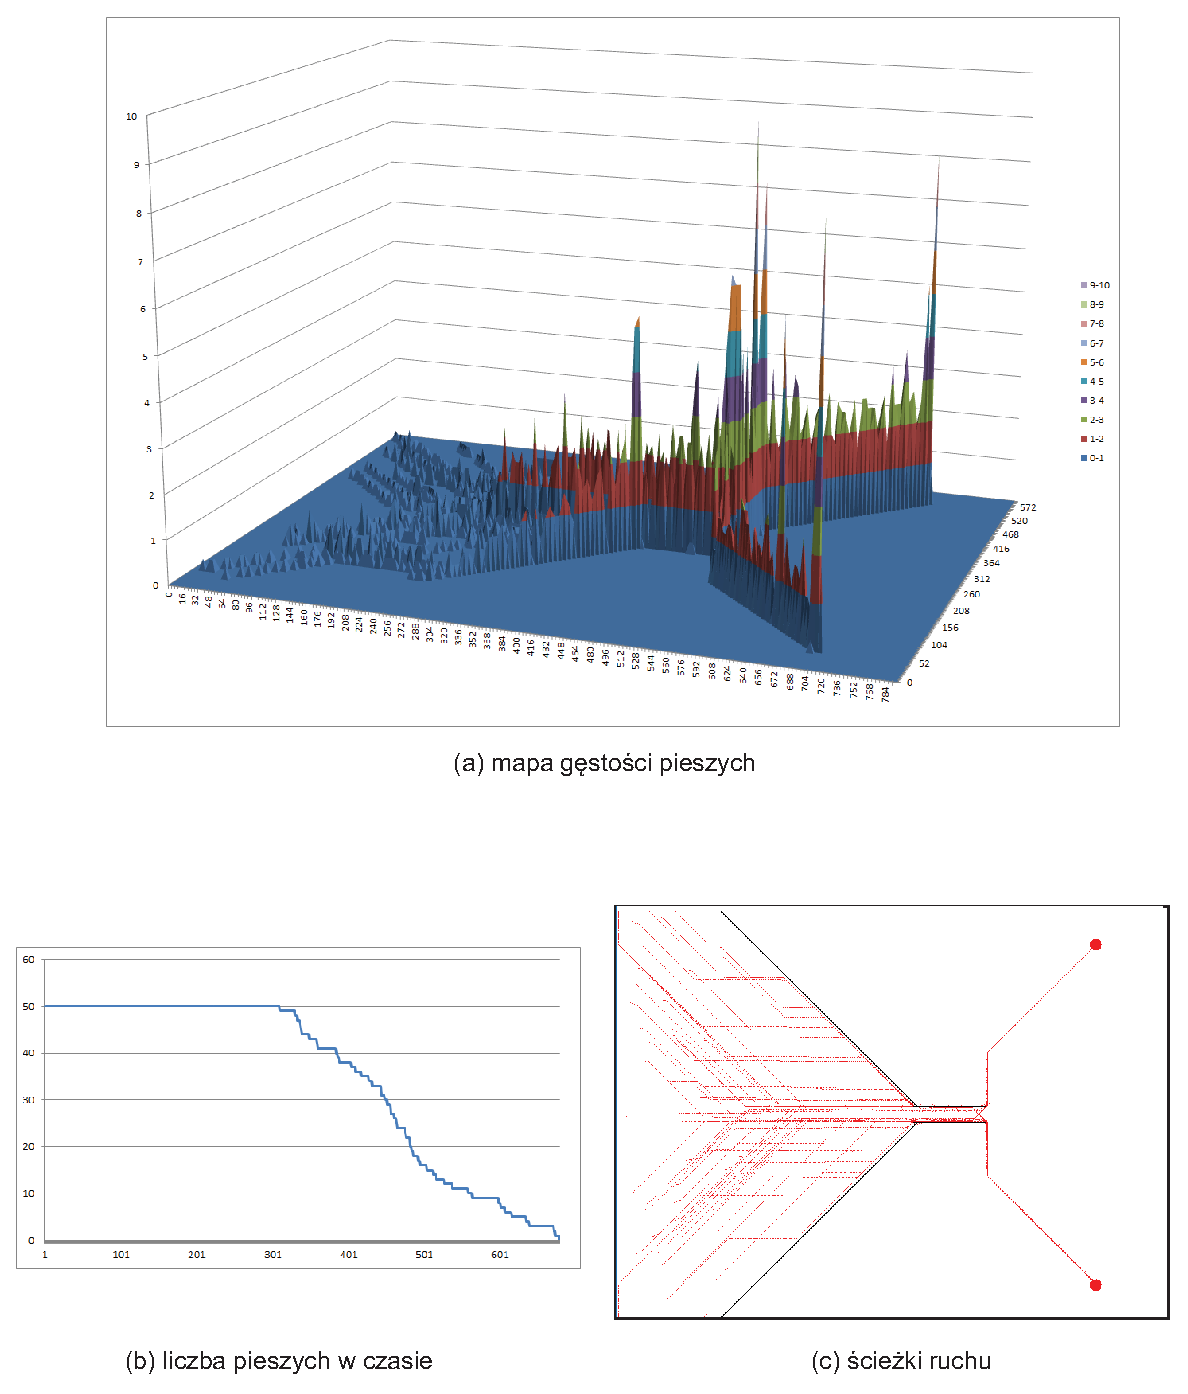
\includegraphics[width=1\textwidth]{lejek50.eps}
\caption{Ruchu pieszych podczas przejścia przez lejek dla 50 agentów, przypadek 5 (opracowanie własne)}
\end{figure}

\begin{figure}
\label{figure:siatka}
\centering
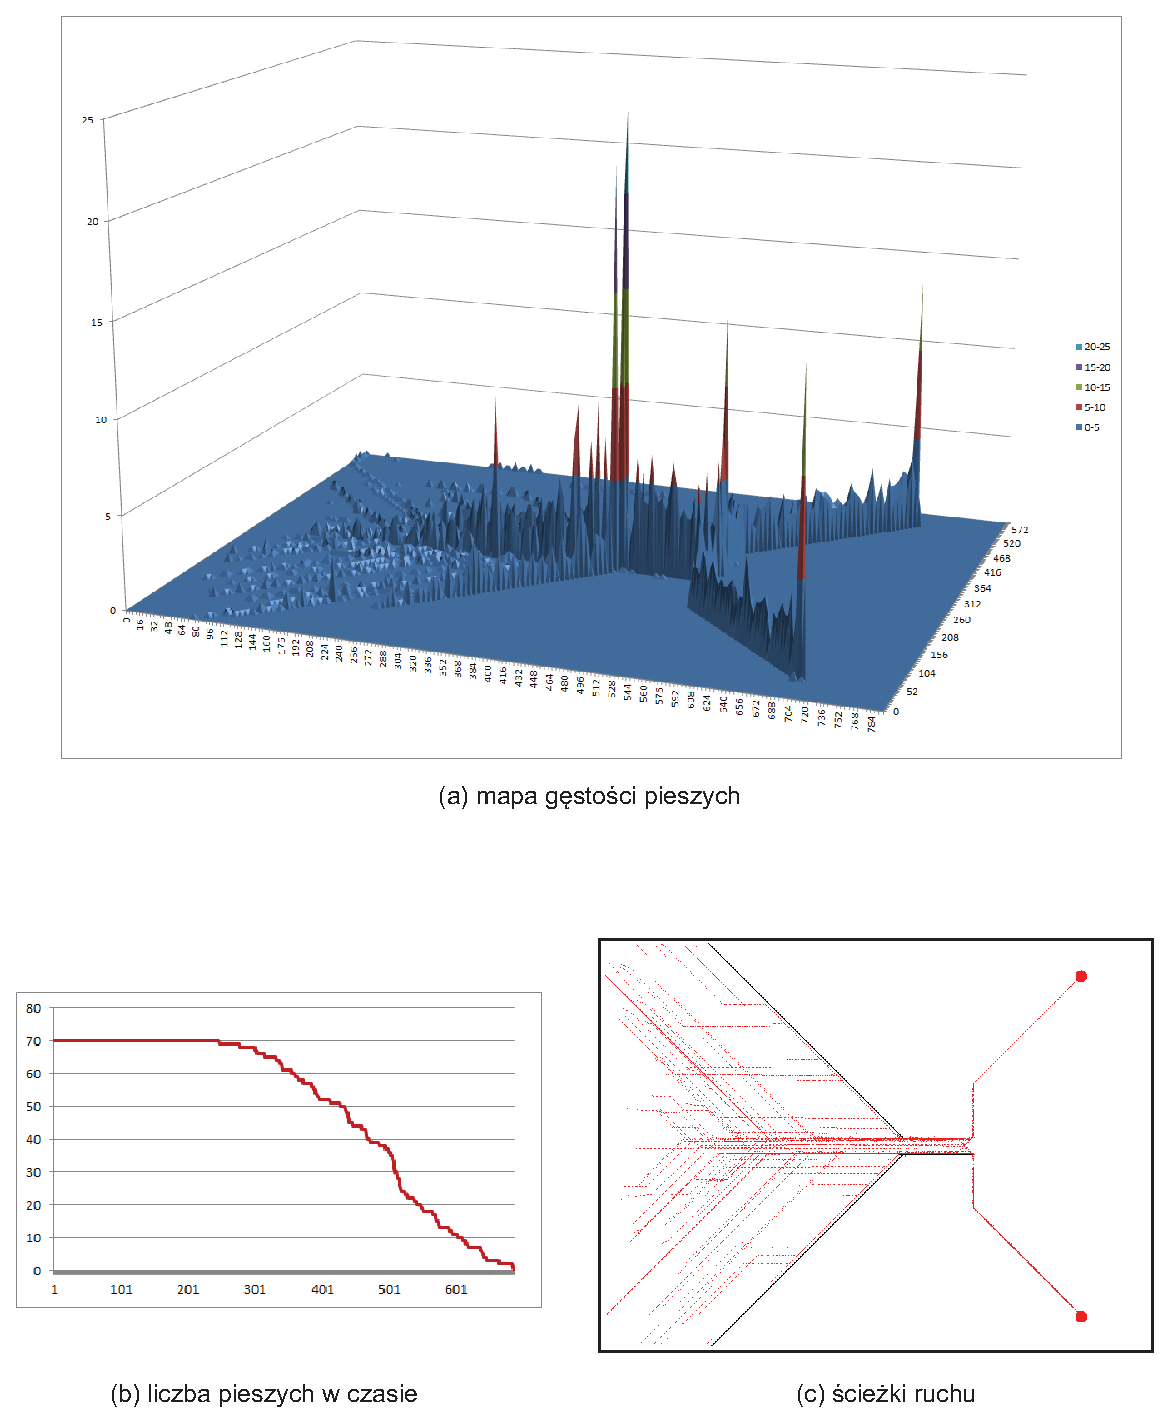
\includegraphics[width=1\textwidth]{lejek70.eps}
\caption{Ruchu pieszych podczas przejścia przez lejek dla 70 agentów, przypadek 5 (opracowanie własne)}
\end{figure}

\begin{figure}
\label{figure:siatka}
\centering
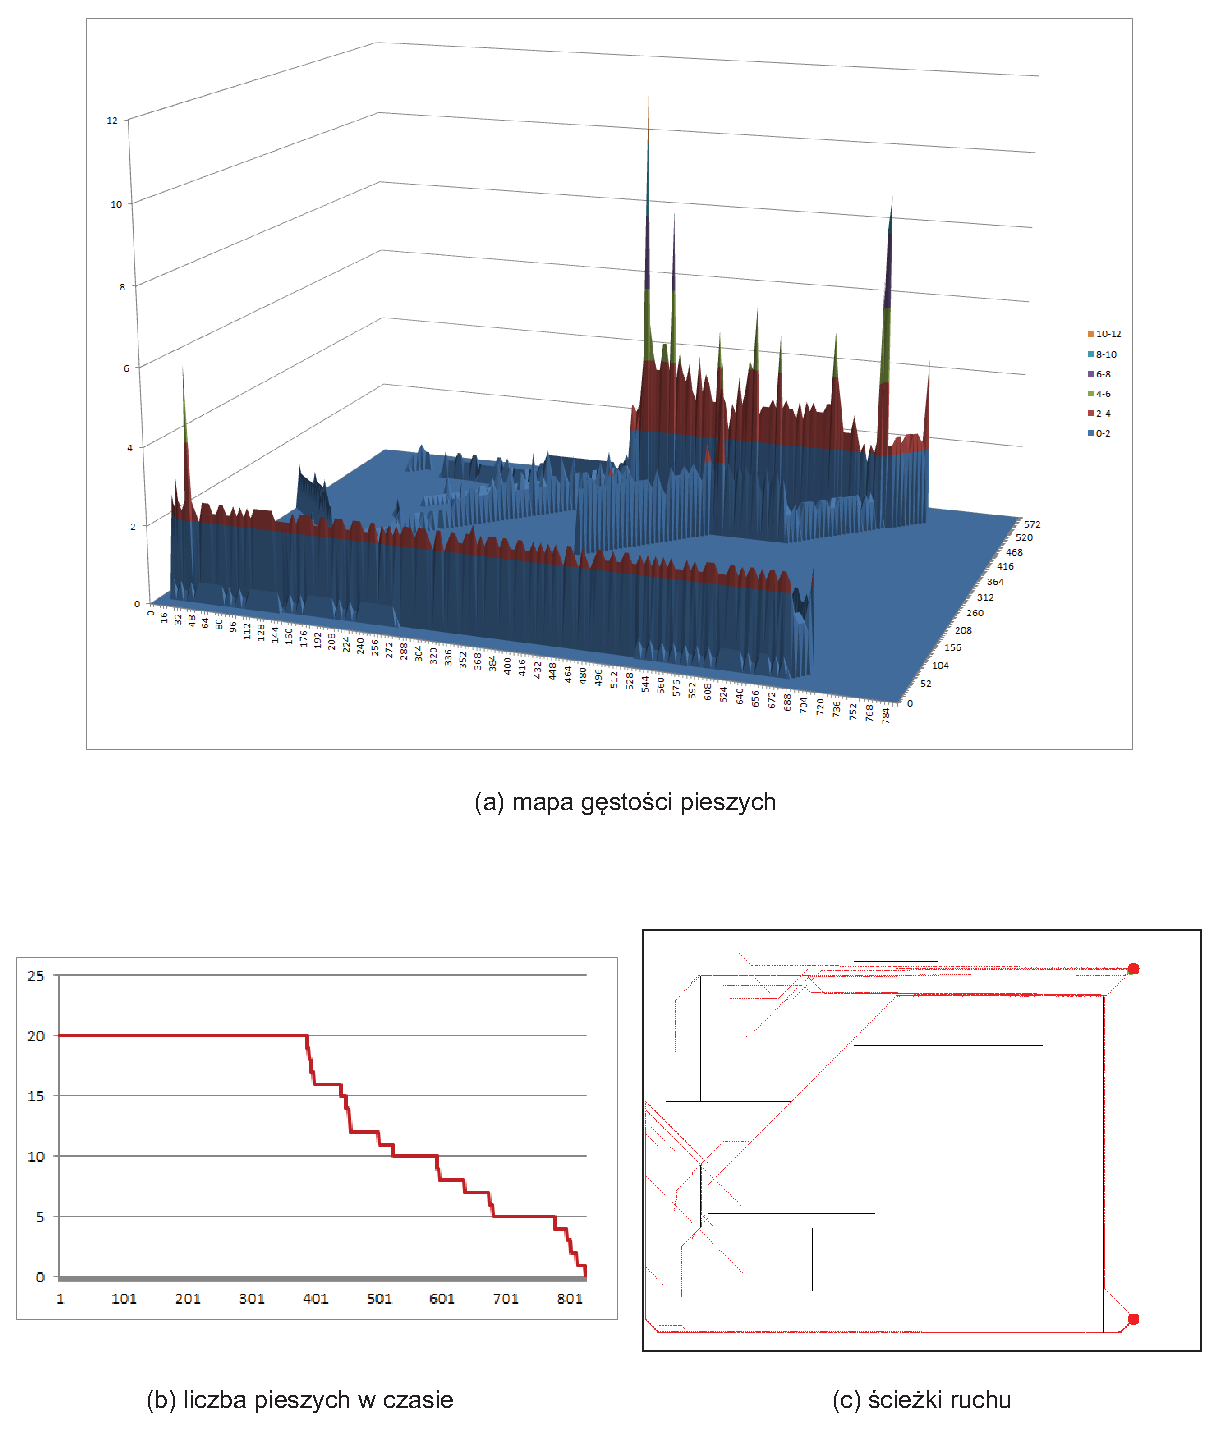
\includegraphics[width=1\textwidth]{maze20.eps}
\caption{Ruchu pieszych podczas przejścia przez labirynt dla 20 agentów, przypadek 6 (opracowanie własne)}
\end{figure}


\begin{figure}
\label{figure:siatka}
\centering
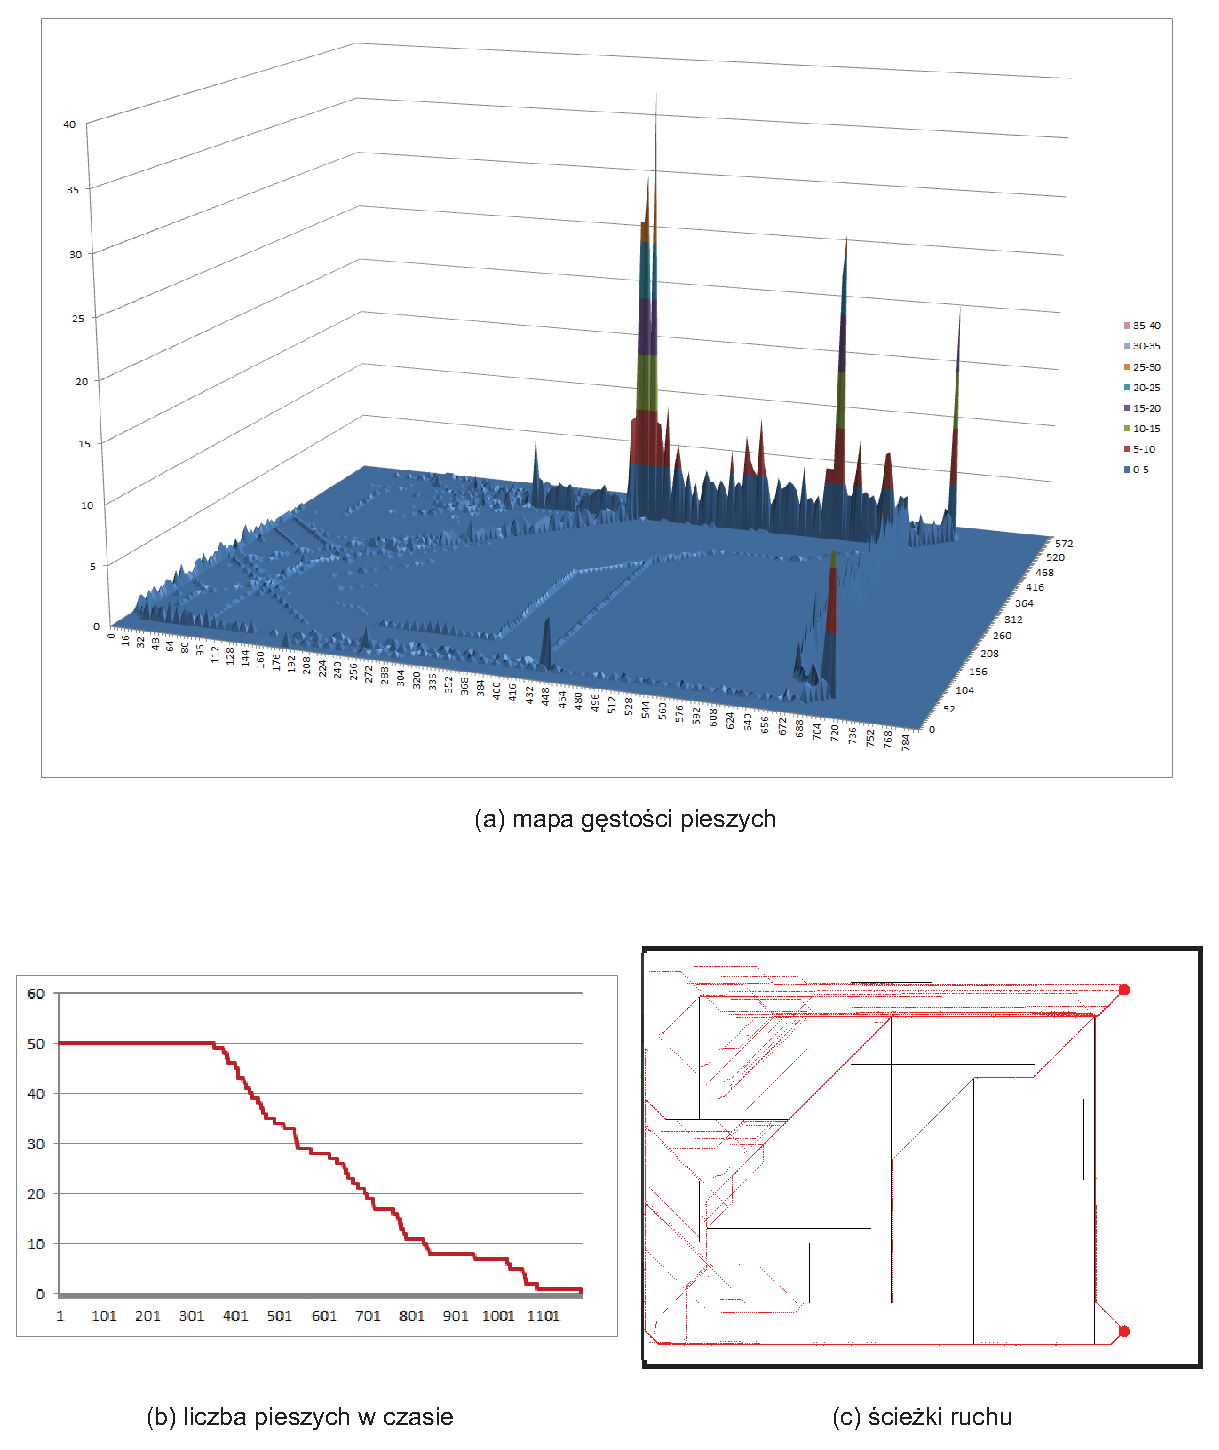
\includegraphics[width=1\textwidth]{maze50.eps}
\caption{Ruchu pieszych podczas przejścia przez labirynt dla 50 agentów, przypadek 7 (opracowanie własne)}
\end{figure}

